\section{方法}


\subsection{使用法,コマンド}
my\_helpからhikiに変換するときのコマンドと使用法は以下の通りである.
\begin{itemize}
\item TARGET --push : 作成したメモ(TARGET)をサーバに送る
\end{itemize}  
\begin{itemize}
\item my\_help --hiki : 作成したメモをhiki形式に変換し,wikiで表示できるようにする.
\end{itemize}

\subsection{TARGET --push のコードの詳述}
TARGET --pushのコードについて詳述する.
\begin{figure}[htbp]\begin{center}
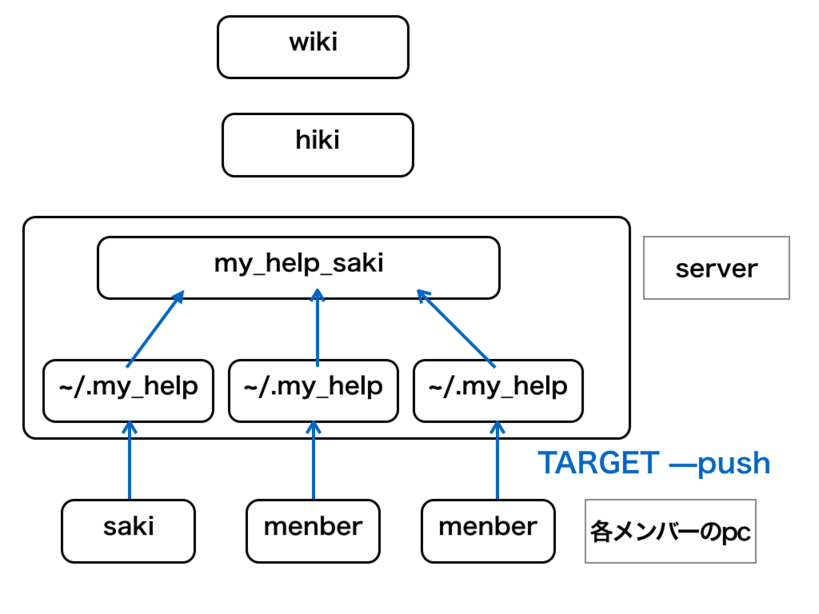
\includegraphics[width=6cm,bb=100 100 600 700]{my_help2hiki_saki.012.png}
\caption{TARGET --push}
\label{default}\end{center}\end{figure}

コードの中身は以下の通りである.
\begin{quote}\begin{verbatim}
    def push                             
      p "push my_todo"
      data_dir = File.join(ENV['HOME'],'.my_help')
      FileUtils.cd(data_dir)
      system "pwd"
      system "rm -rf ~/.my_help/*.yml~"
      system "scp -r ~/.my_help saki@nishitani0:~"
      system "ssh saki@nishitani0 ls ~/.my_help" 
    end
\end{verbatim}\end{quote}

\newpage
コードの詳細を記述する.
\begin{itemize}
\item 3,4行目
\end{itemize}
\begin{description}
\item my\_helpでは,作成したメモが.my\_helpのディレクトリに自動的に追加されるので,
ディレクトリを.my\_helpに移動する.
\end{description}
\begin{itemize}
\item 6行目
\end{itemize}
\begin{description}
\item .my\_helpにメモが追加されるとき,yaml形式のファイルで保存される.
メモを更新すると,一つ前に保存したファイルは*.yml~というファイル名
でバックアップとして残される.
\textbf{rm -rf}で不必要なファイルは削除し,サーバにコピーするときのデータ量を減らしている.
\end{description}

\begin{itemize}
\item 7行目
\end{itemize}
\begin{description}
\item
\textbf{scp -r ~/[directory名] [server名]}
のコマンドによってserverにssh接続を行い,directoryをserverにコピーする.
-rはディレクトリ全体をコピーすることを示している.
西谷研究室で利用しているnishitani0というサーバにコピーしている.
\end{description}

\begin{itemize}
\item 8行目
\end{itemize}
\begin{description}
\item nishitani0にssh接続し.my\_helpの中身を書き出して,
コピーができているかコマンドを実行した時に確認が行えるようにしている.
\end{description}

\newpage

\subsection{my\_help --hiki のコードの詳述}
my\_help --hikのコードについて詳述する.

\begin{figure}[htbp]\begin{center}
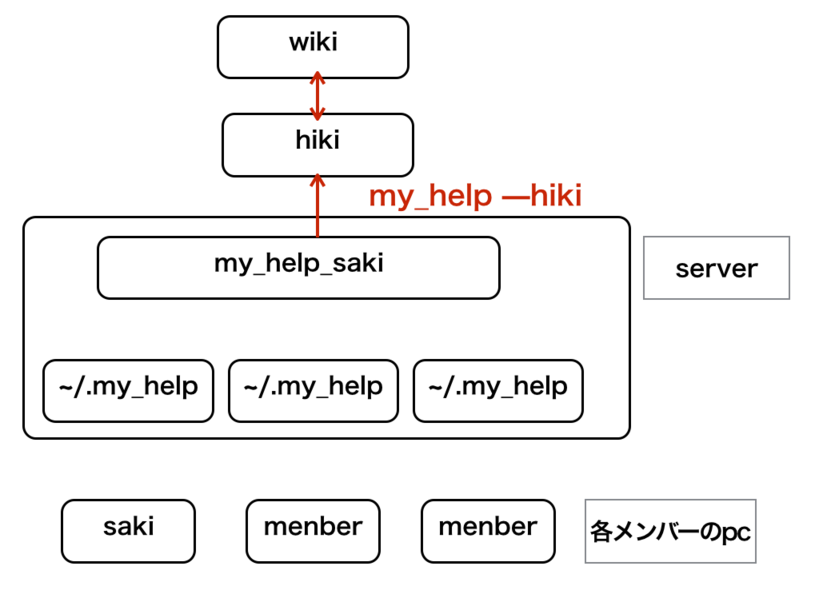
\includegraphics[width=6cm,bb=100 100 600 800]{my_help2hiki_saki.013.png}
\caption{my\_help2hiki}
\label{default}\end{center}\end{figure}

コードの中身は以下の通りである.
\begin{quote}\begin{verbatim}
  def hiki
      p 'my_help2hiki'
      system "emacs_help --to_hiki > ~/Sites/hiki-1.0/data/text/emacs_help_saki"
      system "my_todo --to_hiki > ~/Sites/hiki-1.0/data/text/my_todo_saki"
      system "ssh_help --to_hiki > ~/Sites/hiki-1.0/data/text/ssh_help_saki"
      system "open -a safari 'http://localhost/~saki/hiki-1.0/?FrontPage'"
    end
\end{verbatim}\end{quote}
\newpage
コードの詳細について記述する.
\begin{itemize}
\item 2-4行目
\end{itemize}
\begin{description}
\item my\_helpには,\textbf{TARGET --to\_hiki}というコマンドがあり,これによって
yaml形式で保存されているメモをhiki形式で書き出すことができる.
この --to\_hiki のコマンドを使ってhiki形式にしたものを,wikiで表示することのできる
フォルダである\textbf{~/Sites/hiki-1.0/data/text/}に入れることで,wikiでの表示を可能にしている.
emacs\_help,my\_todo,ssh\_helpは全て私のmy\_helpに入っているメモ.
\end{description}

\begin{itemize}
\item 5行目
\end{itemize}
\begin{description}
\item wikiのページである,図6に示したFrontPageを表示するコマンド.
これによりメモが更新されているのをすぐに確認することができる.
FrontPageは以下のようになっている.
\end{description}
\begin{quote}\begin{verbatim}
!saki's help
*[[ssh_help_saki]]
*[[my_todo_saki]]
*[[emacs_help_saki]]
\end{verbatim}\end{quote}
\begin{description}
\item 先頭に\textbf{!}をつけることで1行目のsaki's helpを見出しにし,
2~4行目は\textbf{*}によって箇条書き,角括弧でリンクになっている.
\end{description}

\begin{figure}[htbp]\begin{center}
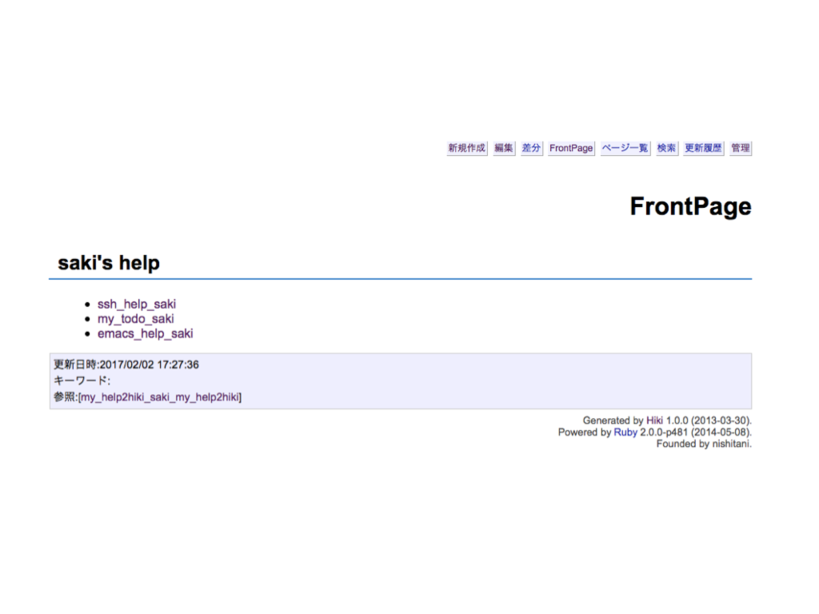
\includegraphics[clip,width=6cm,bb=100 100 600 550]{my_help2hiki_saki.002.png}
\caption{コマンドを実行したときに開くFrontPage }
\label{default}\end{center}\end{figure}

